\chapter{Risultati e Conclusioni}
\label{cha:risultaticonclusioni}

In questo capitolo vengono presentati i principali risultati ottenuti al termine del tirocinio e le 
considerazioni conclusive sull’attività svolta. L’obiettivo è mostrare in che modo la nuova architettura 
implementata abbia migliorato l’efficienza, l’affidabilità e l’osservabilità del processo di calcolo delle 
Community Health Metrics, mettendo in evidenza le differenze rispetto alla soluzione originaria 
basata su uno script monolitico. 

Dopo una breve panoramica dei risultati, corredata da esempi grafici tratti dall’interfaccia di 
Airflow, dalle dashboard di Grafana e dall’applicazione Dash, verranno descritte le competenze acquisite 
e il contributo personale portato al progetto. Infine, saranno discusse le possibili linee di sviluppo futuro 
e le riflessioni conclusive sull’esperienza, sottolineandone l’impatto sia sul piano tecnico sia su quello 
formativo.

\section{Risultati Ottenuti}
\label{sec:risultatiottenuti}

I principali risultati ottenuti al termine del tirocinio possono essere riassunti nei seguenti punti:

\begin{itemize}
    \item \textbf{Modularizzazione del processo di calcolo:} La suddivisione del processo in task distinte ha permesso di migliorare la manutenibilità e la leggibilità del codice, facilitando l’individuazione e la risoluzione di eventuali problemi.
    \item \textbf{Automazione e schedulazione:} L’utilizzo di Apache Airflow ha consentito di automatizzare l’esecuzione del processo, con la possibilità di schedulare le esecuzioni e di monitorare lo stato delle task attraverso un’interfaccia web intuitiva.
    \item \textbf{Containerizzazione:} La containerizzazione della pipeline ha reso possibile l’isolamento delle dipendenze e la standardizzazione dell’ambiente di esecuzione, facilitando il deployment e la scalabilità del sistema. 
    \item \textbf{Monitoraggio e osservabilità:} L’integrazione di Prometheus e Grafana ha permesso di raccogliere metriche dettagliate sul funzionamento della pipeline, offrendo una visione completa delle performance e dello stato del sistema attraverso dashboard personalizzate.
    \item \textbf{Migrazione a PostgreSQL:} La migrazione da SQLite a PostgreSQL ha migliorato la gestione dei dati, garantendo maggiori performance nelle operazioni di lettura e scrittura.
\end{itemize}

Questi risultati hanno portato a un sistema più robusto, efficiente e facile da gestire, in grado di rispondere meglio alle esigenze di calcolo delle Community Health Metrics.
Per dare una dimostrazione concreta dei risultati, si riportano due schermate significative 
relative al funzionamento della nuova architettura.

\begin{figure}[htbp]
    \centering
    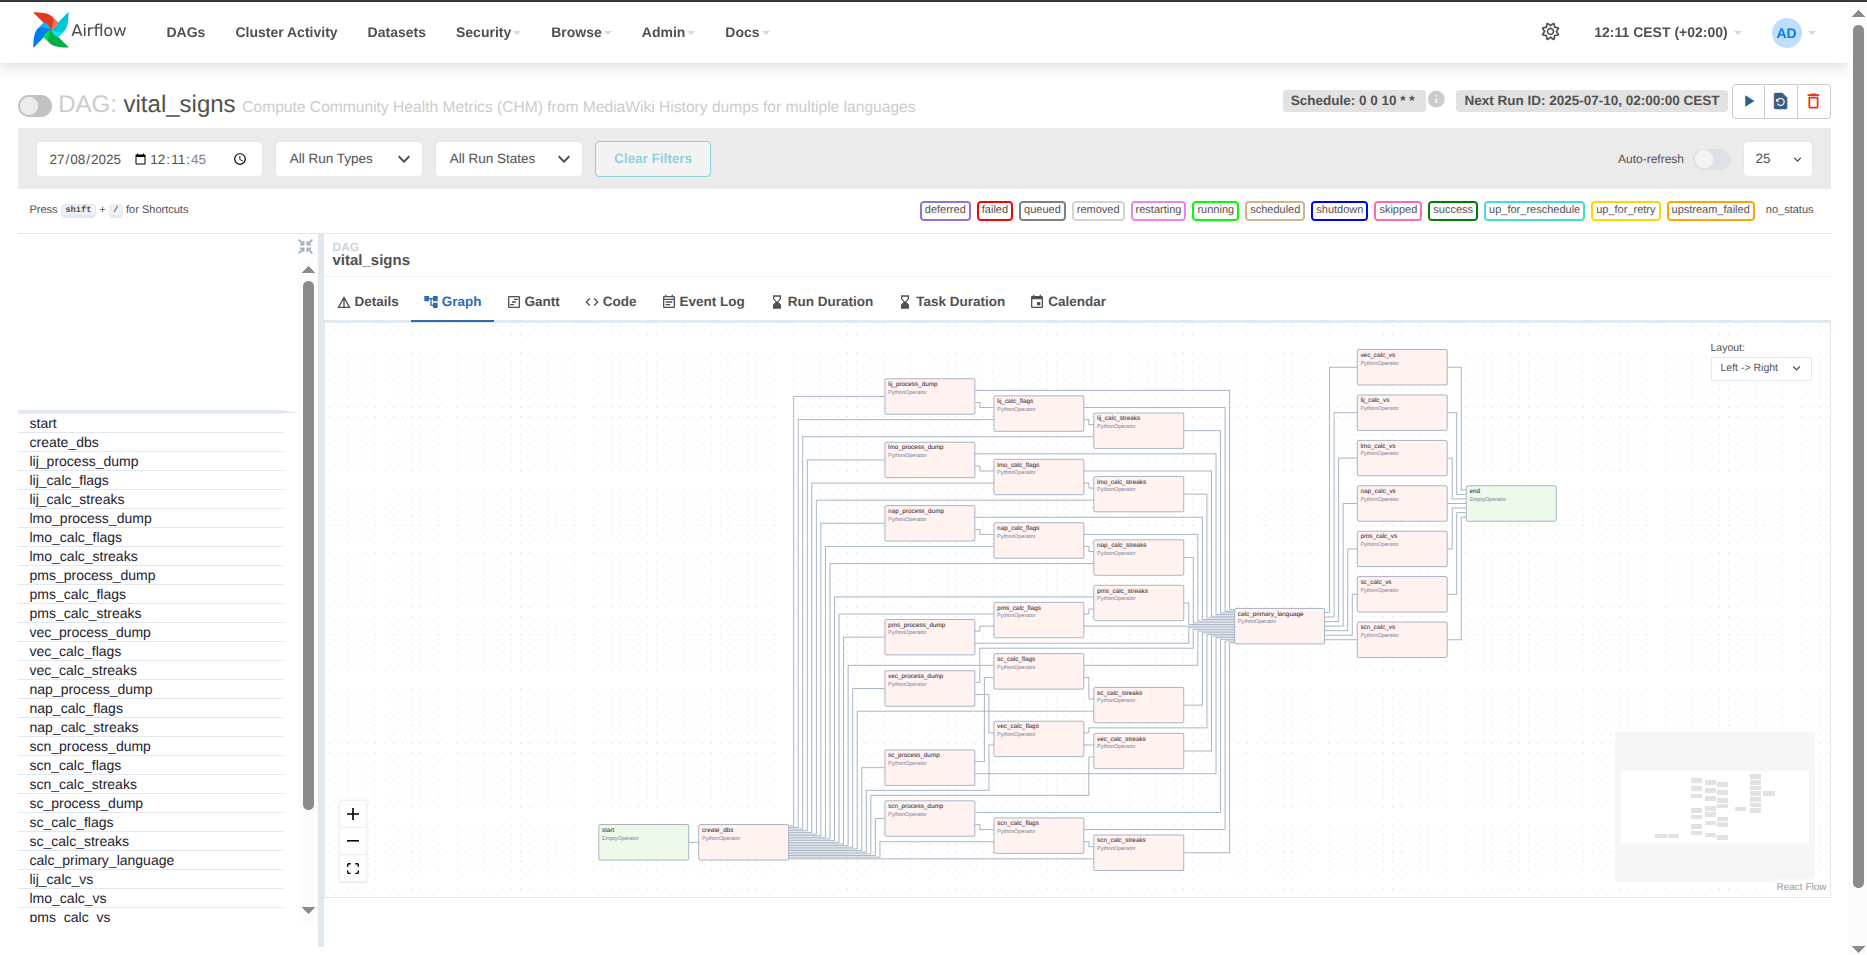
\includegraphics[width=0.9\textwidth]{img/airflowscreen.png}
    \caption{Visualizzazione del DAG nell'interfaccia grafica di Apache Airflow}
    \label{fig:airflowscreen}
\end{figure}

\begin{figure}[htbp]
    \centering
    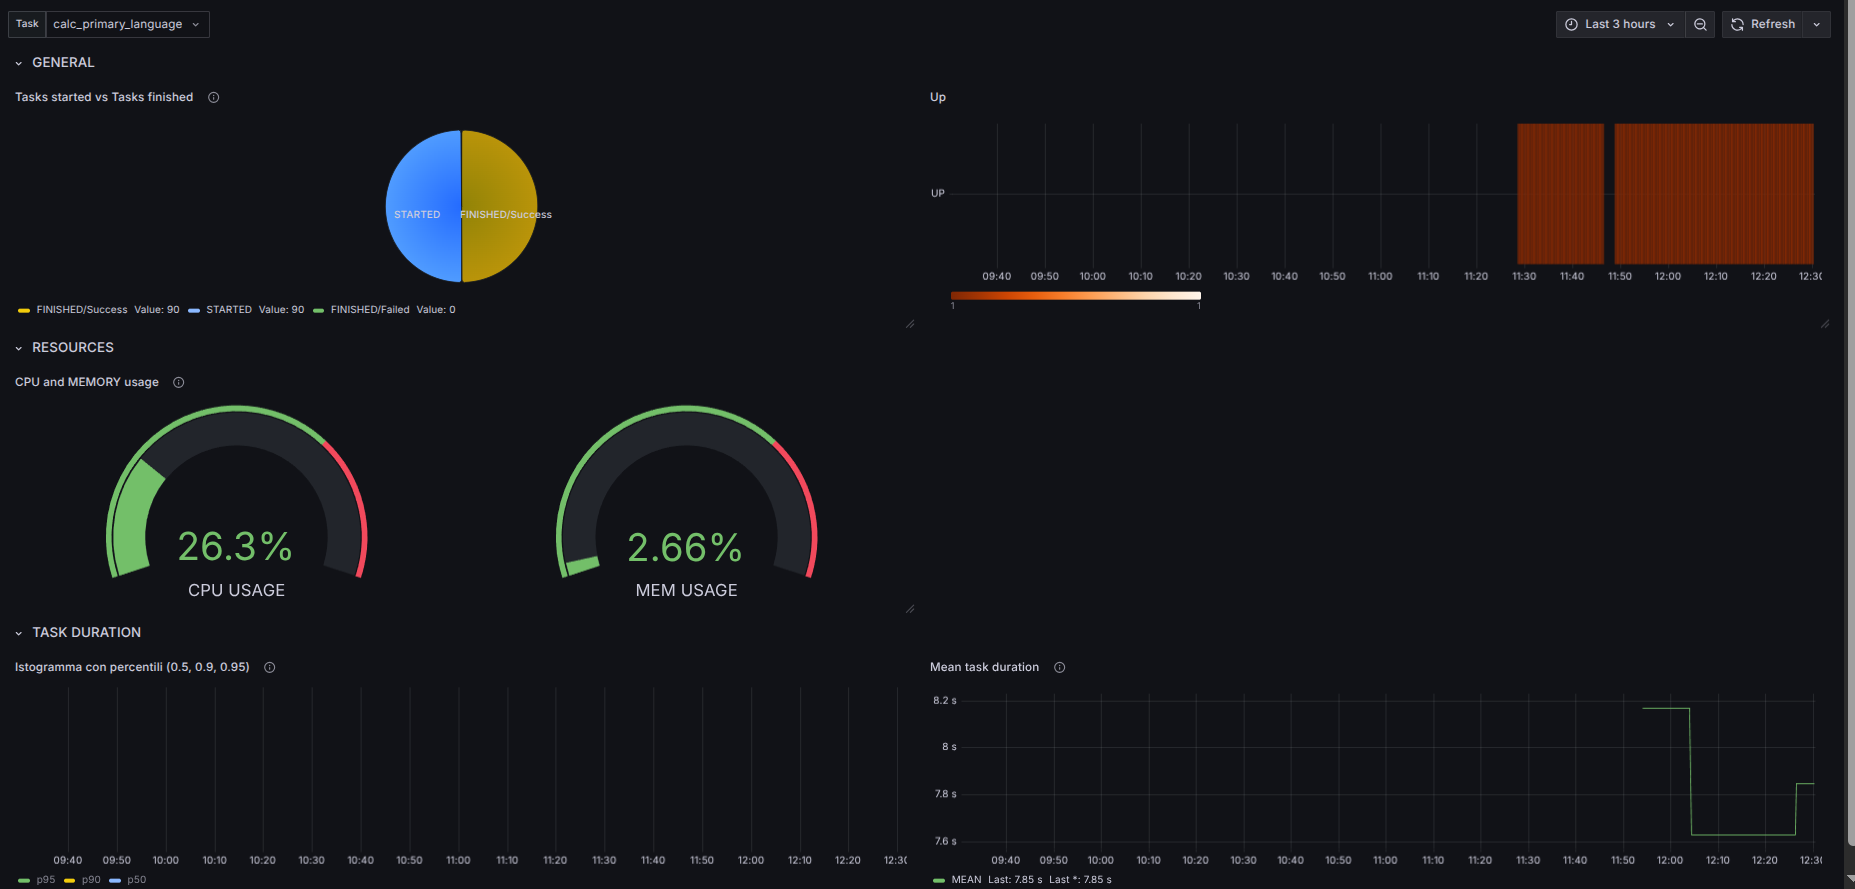
\includegraphics[width=\textwidth]{img/grafanadash.png}
    \caption{Dashboard di monitoraggio realizzata con Grafana}
    \label{fig:grafanadash}
\end{figure}

\newpage



\section{Competenze Acquisite e Contributo Personale}
\label{sec:competenzeacquisitecontributopersonale}

Il tirocinio mi ha permesso di consolidare e ampliare in modo significativo le mie competenze 
nell’ambito dell’ingegneria del software. Il contributo personale si è concentrato sul refactoring 
del codice esistente, sulla progettazione del DAG in Airflow e sulla configurazione dell’infrastruttura 
containerizzata con Docker e docker-compose. 

Dal punto di vista tecnico, le principali competenze acquisite sono state:

\begin{itemize}
    \item \textbf{Python:} durante il progetto ho utilizzato per la prima volta Python in un contesto 
    reale, acquisendo familiarità con la scrittura di script modulari, l’uso di librerie per la manipolazione 
    dei dati e l’integrazione con database tramite SQLAlchemy.
    \item \textbf{SQL e PostgreSQL:} ho approfondito le mie conoscenze di SQL, imparando a scrivere query 
    più complesse e a interagire con un database PostgreSQL, comprendendo le differenze rispetto a SQLite.
    \item \textbf{Docker}: ho imparato a creare immagini Docker personalizzate, a gestire contenitori 
    e a orchestrare più servizi con docker-compose.
    \item \textbf{Apache Airflow:} ho avuto modo di sperimentare per la prima volta uno strumento 
    di orchestrazione di workflow, imparando a definire DAG, gestire dipendenze tra task, 
    configurare la schedulazione e utilizzare l’interfaccia web per il monitoraggio delle esecuzioni.
    \item \textbf{Tecniche di monitoraggio e osservabilità:} ho acquisito conoscenze di base sui concetti 
    di metriche, logging e osservabilità, sperimentando l’integrazione di StatsD, Prometheus e Grafana 
    per la raccolta e la visualizzazione dei dati relativi alle esecuzioni della pipeline.
\end{itemize}

Dal punto di vista personale, l’esperienza mi ha insegnato a lavorare su un progetto esistente 
apprendendo rapidamente tecnologie mai utilizzate prima, a risolvere problemi di integrazione tra 
componenti diversi e a strutturare una pipeline dati modulare e più affidabile. 

\section{Sviluppi Futuri e Considerazioni Conclusive}
\label{sec:sviluppifuturiconsiderazioniconglusive}


Il progetto realizzato durante il tirocinio rappresenta una solida base per ulteriori sviluppi e miglioramenti. Alcune possibili direzioni future includono:
\begin{itemize}
    \item \textbf{Adattamento delle dashboard:} rendere compatibile l’applicazione Dash con il nuovo database PostgreSQL, consentendo la visualizzazione delle Community Health Metrics calcolate dalla pipeline.
    \item \textbf{Deployment delle dashboard:} deployare l’applicazione Dash su un server di produzione, integrandola con l'infrastruttura esistente e garantendo l’accesso sicuro agli utenti.
    \item \textbf{Ottimizzazione delle performance:} analizzare i colli di bottiglia nella pipeline e ottimizzare le performance delle task, ad esempio parallelizzando alcune operazioni o migliorando l’efficienza delle query SQL.
    \item \textbf{Implementazione di alerting:} configurare Prometheus per inviare notifiche in caso di anomalie o fallimenti nelle esecuzioni, migliorando la reattività del sistema.
    \item \textbf{Scalabilità:} esplorare soluzioni per scalare orizzontalmente la pipeline, ad esempio utilizzando Kubernetes per la gestione dei container.
    \item \textbf{Integrazione con altri strumenti:} valutare l’integrazione con altri strumenti di data engineering o machine learning per arricchire le funzionalità della pipeline.
\end{itemize}

In conclusione, il tirocinio ha rappresentato un’esperienza formativa estremamente positiva, permettendomi di acquisire competenze tecniche avanzate e di contribuire a un progetto reale. La nuova architettura implementata ha migliorato notevolmente l’efficienza, l’affidabilità e l’osservabilità del processo di calcolo delle Community Health Metrics, ponendo le basi per ulteriori sviluppi futuri.